\documentclass[1p]{elsarticle_modified}
%\bibliographystyle{elsarticle-num}

%\usepackage[colorlinks]{hyperref}
%\usepackage{abbrmath_seonhwa} %\Abb, \Ascr, \Acal ,\Abf, \Afrak
\usepackage{amsfonts}
\usepackage{amssymb}
\usepackage{amsmath}
\usepackage{amsthm}
\usepackage{scalefnt}
\usepackage{amsbsy}
\usepackage{kotex}
\usepackage{caption}
\usepackage{subfig}
\usepackage{color}
\usepackage{graphicx}
\usepackage{xcolor} %% white, black, red, green, blue, cyan, magenta, yellow
\usepackage{float}
\usepackage{setspace}
\usepackage{hyperref}

\usepackage{tikz}
\usetikzlibrary{arrows}

\usepackage{multirow}
\usepackage{array} % fixed length table
\usepackage{hhline}

%%%%%%%%%%%%%%%%%%%%%
\makeatletter
\renewcommand*\env@matrix[1][\arraystretch]{%
	\edef\arraystretch{#1}%
	\hskip -\arraycolsep
	\let\@ifnextchar\new@ifnextchar
	\array{*\c@MaxMatrixCols c}}
\makeatother %https://tex.stackexchange.com/questions/14071/how-can-i-increase-the-line-spacing-in-a-matrix
%%%%%%%%%%%%%%%

\usepackage[normalem]{ulem}

\newcommand{\msout}[1]{\ifmmode\text{\sout{\ensuremath{#1}}}\else\sout{#1}\fi}
%SOURCE: \msout is \stkout macro in https://tex.stackexchange.com/questions/20609/strikeout-in-math-mode

\newcommand{\cancel}[1]{
	\ifmmode
	{\color{red}\msout{#1}}
	\else
	{\color{red}\sout{#1}}
	\fi
}

\newcommand{\add}[1]{
	{\color{blue}\uwave{#1}}
}

\newcommand{\replace}[2]{
	\ifmmode
	{\color{red}\msout{#1}}{\color{blue}\uwave{#2}}
	\else
	{\color{red}\sout{#1}}{\color{blue}\uwave{#2}}
	\fi
}

\newcommand{\Sol}{\mathcal{S}} %segment
\newcommand{\D}{D} %diagram
\newcommand{\A}{\mathcal{A}} %arc


%%%%%%%%%%%%%%%%%%%%%%%%%%%%%5 test

\def\sl{\operatorname{\textup{SL}}(2,\Cbb)}
\def\psl{\operatorname{\textup{PSL}}(2,\Cbb)}
\def\quan{\mkern 1mu \triangleright \mkern 1mu}

\theoremstyle{definition}
\newtheorem{thm}{Theorem}[section]
\newtheorem{prop}[thm]{Proposition}
\newtheorem{lem}[thm]{Lemma}
\newtheorem{ques}[thm]{Question}
\newtheorem{cor}[thm]{Corollary}
\newtheorem{defn}[thm]{Definition}
\newtheorem{exam}[thm]{Example}
\newtheorem{rmk}[thm]{Remark}
\newtheorem{alg}[thm]{Algorithm}

\newcommand{\I}{\sqrt{-1}}
\begin{document}

%\begin{frontmatter}
%
%\title{Boundary parabolic representations of knots up to 8 crossings}
%
%%% Group authors per affiliation:
%\author{Yunhi Cho} 
%\address{Department of Mathematics, University of Seoul, Seoul, Korea}
%\ead{yhcho@uos.ac.kr}
%
%
%\author{Seonhwa Kim} %\fnref{s_kim}}
%\address{Center for Geometry and Physics, Institute for Basic Science, Pohang, 37673, Korea}
%\ead{ryeona17@ibs.re.kr}
%
%\author{Hyuk Kim}
%\address{Department of Mathematical Sciences, Seoul National University, Seoul 08826, Korea}
%\ead{hyukkim@snu.ac.kr}
%
%\author{Seokbeom Yoon}
%\address{Department of Mathematical Sciences, Seoul National University, Seoul, 08826,  Korea}
%\ead{sbyoon15@snu.ac.kr}
%
%\begin{abstract}
%We find all boundary parabolic representation of knots up to 8 crossings.
%
%\end{abstract}
%\begin{keyword}
%    \MSC[2010] 57M25 
%\end{keyword}
%
%\end{frontmatter}

%\linenumbers
%\tableofcontents
%
\newcommand\colored[1]{\textcolor{white}{\rule[-0.35ex]{0.8em}{1.4ex}}\kern-0.8em\color{red} #1}%
%\newcommand\colored[1]{\textcolor{white}{ #1}\kern-2.17ex	\textcolor{white}{ #1}\kern-1.81ex	\textcolor{white}{ #1}\kern-2.15ex\color{red}#1	}

{\Large $\underline{12a_{0223}~(K12a_{0223})}$}

\setlength{\tabcolsep}{10pt}
\renewcommand{\arraystretch}{1.6}
\vspace{1cm}\begin{tabular}{m{100pt}>{\centering\arraybackslash}m{274pt}}
\multirow{5}{120pt}{
	\centering
	\includegraphics[width=112pt]{../../../GIT/diagram.site/Diagrams/png/1024_12a_0223.png}\\
\ \ \ A knot diagram\footnotemark}&
\allowdisplaybreaks
\textbf{Linearized knot diagam} \\
\cline{2-2}
 &
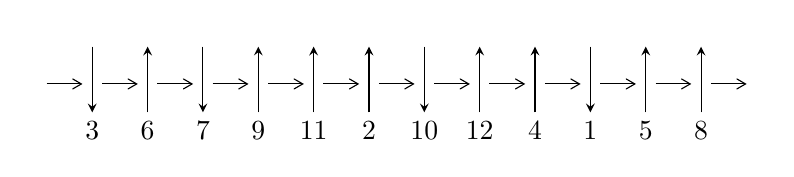
\begin{tikzpicture}[x=20pt, y=17pt]
	% nodes
	\node (C0) at (0, 0) {};
	\node (C1) at (1, 0) {};
	\node (C1U) at (1, +1) {};
	\node (C1D) at (1, -1) {3};

	\node (C2) at (2, 0) {};
	\node (C2U) at (2, +1) {};
	\node (C2D) at (2, -1) {6};

	\node (C3) at (3, 0) {};
	\node (C3U) at (3, +1) {};
	\node (C3D) at (3, -1) {7};

	\node (C4) at (4, 0) {};
	\node (C4U) at (4, +1) {};
	\node (C4D) at (4, -1) {9};

	\node (C5) at (5, 0) {};
	\node (C5U) at (5, +1) {};
	\node (C5D) at (5, -1) {11};

	\node (C6) at (6, 0) {};
	\node (C6U) at (6, +1) {};
	\node (C6D) at (6, -1) {2};

	\node (C7) at (7, 0) {};
	\node (C7U) at (7, +1) {};
	\node (C7D) at (7, -1) {10};

	\node (C8) at (8, 0) {};
	\node (C8U) at (8, +1) {};
	\node (C8D) at (8, -1) {12};

	\node (C9) at (9, 0) {};
	\node (C9U) at (9, +1) {};
	\node (C9D) at (9, -1) {4};

	\node (C10) at (10, 0) {};
	\node (C10U) at (10, +1) {};
	\node (C10D) at (10, -1) {1};

	\node (C11) at (11, 0) {};
	\node (C11U) at (11, +1) {};
	\node (C11D) at (11, -1) {5};

	\node (C12) at (12, 0) {};
	\node (C12U) at (12, +1) {};
	\node (C12D) at (12, -1) {8};
	\node (C13) at (13, 0) {};

	% arrows
	\draw[->,>={angle 60}]
	(C0) edge (C1) (C1) edge (C2) (C2) edge (C3) (C3) edge (C4) (C4) edge (C5) (C5) edge (C6) (C6) edge (C7) (C7) edge (C8) (C8) edge (C9) (C9) edge (C10) (C10) edge (C11) (C11) edge (C12) (C12) edge (C13) ;	\draw[->,>=stealth]
	(C1U) edge (C1D) (C2D) edge (C2U) (C3U) edge (C3D) (C4D) edge (C4U) (C5D) edge (C5U) (C6D) edge (C6U) (C7U) edge (C7D) (C8D) edge (C8U) (C9D) edge (C9U) (C10U) edge (C10D) (C11D) edge (C11U) (C12D) edge (C12U) ;
	\end{tikzpicture} \\
\hhline{~~} \\& 
\textbf{Solving Sequence} \\ \cline{2-2} 
 &
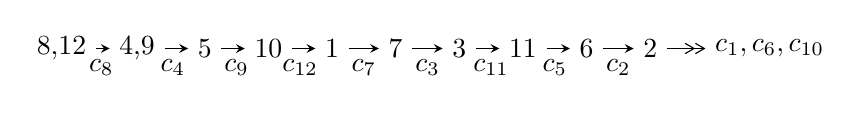
\begin{tikzpicture}[x=23pt, y=7pt]
	% node
	\node (A0) at (-1/8, 0) {8,12};
	\node (A1) at (17/16, 0) {4,9};
	\node (A2) at (17/8, 0) {5};
	\node (A3) at (25/8, 0) {10};
	\node (A4) at (33/8, 0) {1};
	\node (A5) at (41/8, 0) {7};
	\node (A6) at (49/8, 0) {3};
	\node (A7) at (57/8, 0) {11};
	\node (A8) at (65/8, 0) {6};
	\node (A9) at (73/8, 0) {2};
	\node (C1) at (1/2, -1) {$c_{8}$};
	\node (C2) at (13/8, -1) {$c_{4}$};
	\node (C3) at (21/8, -1) {$c_{9}$};
	\node (C4) at (29/8, -1) {$c_{12}$};
	\node (C5) at (37/8, -1) {$c_{7}$};
	\node (C6) at (45/8, -1) {$c_{3}$};
	\node (C7) at (53/8, -1) {$c_{11}$};
	\node (C8) at (61/8, -1) {$c_{5}$};
	\node (C9) at (69/8, -1) {$c_{2}$};
	\node (A10) at (11, 0) {$c_{1},c_{6},c_{10}$};

	% edge
	\draw[->,>=stealth]	
	(A0) edge (A1) (A1) edge (A2) (A2) edge (A3) (A3) edge (A4) (A4) edge (A5) (A5) edge (A6) (A6) edge (A7) (A7) edge (A8) (A8) edge (A9) ;
	\draw[->>,>={angle 60}]	
	(A9) edge (A10);
\end{tikzpicture} \\ 

\end{tabular} \\

\footnotetext{
The image of knot diagram is generated by the software ``\textbf{Draw programme}" developed by Andrew Bartholomew(\url{http://www.layer8.co.uk/maths/draw/index.htm\#Running-draw}), where we modified some parts for our purpose(\url{https://github.com/CATsTAILs/LinksPainter}).
}\phantom \\ \newline 
\centering \textbf{Ideals for irreducible components\footnotemark of $X_{\text{par}}$} 
 
\begin{align*}
I^u_{1}&=\langle 
769 u^{45}+22195 u^{44}+\cdots+2048 b+18618368,\;-1645 u^{45}-50133 u^{44}+\cdots+8192 a-21766144,\\
\phantom{I^u_{1}}&\phantom{= \langle  }u^{46}+29 u^{45}+\cdots+172032 u+8192\rangle \\
I^u_{2}&=\langle 
-5.15204\times10^{18} a^{19} u^{2}-9.61919\times10^{18} a^{18} u^{2}+\cdots-5.70417\times10^{21} a-2.02099\times10^{21},\\
\phantom{I^u_{2}}&\phantom{= \langle  }-2 a^{19} u^2-5 a^{18} u^2+\cdots+389 a+155,\;u^3- u^2+2 u-1\rangle \\
I^u_{3}&=\langle 
4 u^{29}+u^{28}+\cdots+b+33,\;-29 u^{29}+70 u^{28}+\cdots+2 a-55,\;u^{30}-2 u^{29}+\cdots+u+2\rangle \\
I^u_{4}&=\langle 
67 a^5 u^2+102 a^4 u^2+\cdots+362 a+422,\;-2 a^4 u^2-2 a^3 u^2+\cdots-11 a+1,\;u^3- u^2+2 u-1\rangle \\
\\
\end{align*}
\raggedright * 4 irreducible components of $\dim_{\mathbb{C}}=0$, with total 154 representations.\\
\footnotetext{All coefficients of polynomials are rational numbers. But the coefficients are sometimes approximated in decimal forms when there is not enough margin.}
\newpage
\renewcommand{\arraystretch}{1}
\centering \section*{I. $I^u_{1}= \langle 769 u^{45}+22195 u^{44}+\cdots+2048 b+18618368,\;-1645 u^{45}-5.01\times10^{4} u^{44}+\cdots+8192 a-2.18\times10^{7},\;u^{46}+29 u^{45}+\cdots+172032 u+8192 \rangle$}
\flushleft \textbf{(i) Arc colorings}\\
\begin{tabular}{m{7pt} m{180pt} m{7pt} m{180pt} }
\flushright $a_{8}=$&$\begin{pmatrix}1\\0\end{pmatrix}$ \\
\flushright $a_{12}=$&$\begin{pmatrix}0\\u\end{pmatrix}$ \\
\flushright $a_{4}=$&$\begin{pmatrix}0.200806 u^{45}+6.11975 u^{44}+\cdots+46599.5 u+2657\\-0.375488 u^{45}-10.8374 u^{44}+\cdots-180404 u-9091\end{pmatrix}$ \\
\flushright $a_{9}=$&$\begin{pmatrix}1\\- u^2\end{pmatrix}$ \\
\flushright $a_{5}=$&$\begin{pmatrix}-1.40613 u^{45}-39.1708 u^{44}+\cdots-186438. u-8862\\-0.296387 u^{45}-7.36377 u^{44}+\cdots+31888 u+1645\end{pmatrix}$ \\
\flushright $a_{10}=$&$\begin{pmatrix}\frac{1}{8192} u^{45}+\frac{119}{8192} u^{44}+\cdots+933 u+46\\0.505615 u^{45}+14.1682 u^{44}+\cdots+82866 u+4141\end{pmatrix}$ \\
\flushright $a_{1}=$&$\begin{pmatrix}u\\u\end{pmatrix}$ \\
\flushright $a_{7}=$&$\begin{pmatrix}-0.274048 u^{45}-7.68079 u^{44}+\cdots-42145.5 u-2100\\0.982910 u^{45}+27.7881 u^{44}+\cdots+203839 u+10297\end{pmatrix}$ \\
\flushright $a_{3}=$&$\begin{pmatrix}-2.30249 u^{45}-65.0942 u^{44}+\cdots-648664. u-33111\\1.45679 u^{45}+41.2253 u^{44}+\cdots+186450 u+9592\end{pmatrix}$ \\
\flushright $a_{11}=$&$\begin{pmatrix}-0.494507 u^{45}-13.8463 u^{44}+\cdots-81908 u-4096\\\frac{45}{4096} u^{45}+\frac{1259}{4096} u^{44}+\cdots+25 u-1\end{pmatrix}$ \\
\flushright $a_{6}=$&$\begin{pmatrix}-2.72314 u^{45}-76.9080 u^{44}+\cdots-541748. u-26895\\0.812256 u^{45}+23.5637 u^{44}+\cdots+155986 u+7758\end{pmatrix}$ \\
\flushright $a_{2}=$&$\begin{pmatrix}-5.37744 u^{45}-152.656 u^{44}+\cdots-1.53361\times10^{6} u-79260.5\\1.09839 u^{45}+31.0549 u^{44}+\cdots+140452. u+7392\end{pmatrix}$\\&\end{tabular}
\flushleft \textbf{(ii) Obstruction class $= -1$}\\~\\
\flushleft \textbf{(iii) Cusp Shapes $= -\frac{5013}{1024} u^{45}-\frac{144727}{1024} u^{44}+\cdots-1843566 u-96850$}\\~\\
\newpage\renewcommand{\arraystretch}{1}
\flushleft \textbf{(iv) u-Polynomials at the component}\newline \\
\begin{tabular}{m{50pt}|m{274pt}}
Crossings & \hspace{64pt}u-Polynomials at each crossing \\
\hline $$\begin{aligned}c_{1}\end{aligned}$$&$\begin{aligned}
&u^{46}+23 u^{45}+\cdots+160 u+64
\end{aligned}$\\
\hline $$\begin{aligned}c_{2},c_{6}\end{aligned}$$&$\begin{aligned}
&u^{46}-9 u^{45}+\cdots-80 u+8
\end{aligned}$\\
\hline $$\begin{aligned}c_{3}\end{aligned}$$&$\begin{aligned}
&u^{46}+9 u^{45}+\cdots+48000 u+8768
\end{aligned}$\\
\hline $$\begin{aligned}c_{4},c_{5},c_{9}\\c_{11}\end{aligned}$$&$\begin{aligned}
&u^{46}+22 u^{44}+\cdots+2 u+1
\end{aligned}$\\
\hline $$\begin{aligned}c_{7},c_{10}\end{aligned}$$&$\begin{aligned}
&u^{46}-3 u^{45}+\cdots+15 u+1
\end{aligned}$\\
\hline $$\begin{aligned}c_{8},c_{12}\end{aligned}$$&$\begin{aligned}
&u^{46}-29 u^{45}+\cdots-172032 u+8192
\end{aligned}$\\
\hline
\end{tabular}\\~\\
\newpage\renewcommand{\arraystretch}{1}
\flushleft \textbf{(v) Riley Polynomials at the component}\newline \\
\begin{tabular}{m{50pt}|m{274pt}}
Crossings & \hspace{64pt}Riley Polynomials at each crossing \\
\hline $$\begin{aligned}c_{1}\end{aligned}$$&$\begin{aligned}
&y^{46}+3 y^{45}+\cdots+34304 y+4096
\end{aligned}$\\
\hline $$\begin{aligned}c_{2},c_{6}\end{aligned}$$&$\begin{aligned}
&y^{46}+23 y^{45}+\cdots+160 y+64
\end{aligned}$\\
\hline $$\begin{aligned}c_{3}\end{aligned}$$&$\begin{aligned}
&y^{46}-17 y^{45}+\cdots+657339392 y+76877824
\end{aligned}$\\
\hline $$\begin{aligned}c_{4},c_{5},c_{9}\\c_{11}\end{aligned}$$&$\begin{aligned}
&y^{46}+44 y^{45}+\cdots+2 y+1
\end{aligned}$\\
\hline $$\begin{aligned}c_{7},c_{10}\end{aligned}$$&$\begin{aligned}
&y^{46}-21 y^{45}+\cdots-131 y+1
\end{aligned}$\\
\hline $$\begin{aligned}c_{8},c_{12}\end{aligned}$$&$\begin{aligned}
&y^{46}+23 y^{45}+\cdots-301989888 y+67108864
\end{aligned}$\\
\hline
\end{tabular}\\~\\
\newpage\flushleft \textbf{(vi) Complex Volumes and Cusp Shapes}
$$\begin{array}{c|c|c}  
\text{Solutions to }I^u_{1}& \I (\text{vol} + \sqrt{-1}CS) & \text{Cusp shape}\\
 \hline 
\begin{aligned}
u &= -0.799771 + 0.573925 I \\
a &= \phantom{-}0.364393 + 0.335556 I \\
b &= -0.066790 - 0.489318 I\end{aligned}
 & \phantom{-}0.23982 - 5.32921 I & \phantom{-0.000000 } 0 \\ \hline\begin{aligned}
u &= -0.799771 - 0.573925 I \\
a &= \phantom{-}0.364393 - 0.335556 I \\
b &= -0.066790 + 0.489318 I\end{aligned}
 & \phantom{-}0.23982 + 5.32921 I & \phantom{-0.000000 } 0 \\ \hline\begin{aligned}
u &= \phantom{-}0.893801 + 0.251608 I \\
a &= \phantom{-}0.044626 + 1.229910 I \\
b &= \phantom{-}0.58367 - 1.51957 I\end{aligned}
 & \phantom{-}1.15969 + 2.64455 I & \phantom{-0.000000 } 0 \\ \hline\begin{aligned}
u &= \phantom{-}0.893801 - 0.251608 I \\
a &= \phantom{-}0.044626 - 1.229910 I \\
b &= \phantom{-}0.58367 + 1.51957 I\end{aligned}
 & \phantom{-}1.15969 - 2.64455 I & \phantom{-0.000000 } 0 \\ \hline\begin{aligned}
u &= -0.512458 + 0.963987 I \\
a &= -0.430313 + 0.180490 I \\
b &= -0.0655666 - 0.0544458 I\end{aligned}
 & \phantom{-}0.14368 - 3.22065 I & \phantom{-0.000000 } 0 \\ \hline\begin{aligned}
u &= -0.512458 - 0.963987 I \\
a &= -0.430313 - 0.180490 I \\
b &= -0.0655666 + 0.0544458 I\end{aligned}
 & \phantom{-}0.14368 + 3.22065 I & \phantom{-0.000000 } 0 \\ \hline\begin{aligned}
u &= -0.388129 + 1.023260 I \\
a &= -0.426674 + 0.589584 I \\
b &= -0.183361 + 0.160958 I\end{aligned}
 & -1.19630 - 3.09642 I & \phantom{-0.000000 } 0 \\ \hline\begin{aligned}
u &= -0.388129 - 1.023260 I \\
a &= -0.426674 - 0.589584 I \\
b &= -0.183361 - 0.160958 I\end{aligned}
 & -1.19630 + 3.09642 I & \phantom{-0.000000 } 0 \\ \hline\begin{aligned}
u &= -0.324185 + 1.064380 I \\
a &= \phantom{-}0.399633 - 0.786327 I \\
b &= \phantom{-}0.197166 - 0.347962 I\end{aligned}
 & -4.51131 + 0.55103 I & \phantom{-0.000000 } 0 \\ \hline\begin{aligned}
u &= -0.324185 - 1.064380 I \\
a &= \phantom{-}0.399633 + 0.786327 I \\
b &= \phantom{-}0.197166 + 0.347962 I\end{aligned}
 & -4.51131 - 0.55103 I & \phantom{-0.000000 } 0\\
 \hline 
 \end{array}$$\newpage$$\begin{array}{c|c|c}  
\text{Solutions to }I^u_{1}& \I (\text{vol} + \sqrt{-1}CS) & \text{Cusp shape}\\
 \hline 
\begin{aligned}
u &= -0.636420 + 0.928507 I \\
a &= \phantom{-}0.487473 + 0.128530 I \\
b &= -0.118282 + 0.098125 I\end{aligned}
 & -0.796799 + 0.099834 I & \phantom{-0.000000 } 0 \\ \hline\begin{aligned}
u &= -0.636420 - 0.928507 I \\
a &= \phantom{-}0.487473 - 0.128530 I \\
b &= -0.118282 - 0.098125 I\end{aligned}
 & -0.796799 - 0.099834 I & \phantom{-0.000000 } 0 \\ \hline\begin{aligned}
u &= -0.400449 + 1.071460 I \\
a &= \phantom{-}0.563394 - 0.645136 I \\
b &= \phantom{-}0.312197 - 0.165596 I\end{aligned}
 & -4.04848 - 7.39004 I & \phantom{-0.000000 } 0 \\ \hline\begin{aligned}
u &= -0.400449 - 1.071460 I \\
a &= \phantom{-}0.563394 + 0.645136 I \\
b &= \phantom{-}0.312197 + 0.165596 I\end{aligned}
 & -4.04848 + 7.39004 I & \phantom{-0.000000 } 0 \\ \hline\begin{aligned}
u &= -0.065239 + 0.801819 I \\
a &= \phantom{-}0.118295 + 0.879729 I \\
b &= \phantom{-}0.403205 + 0.174145 I\end{aligned}
 & -1.90599 - 1.35920 I & \phantom{-0.000000 } 0 \\ \hline\begin{aligned}
u &= -0.065239 - 0.801819 I \\
a &= \phantom{-}0.118295 - 0.879729 I \\
b &= \phantom{-}0.403205 - 0.174145 I\end{aligned}
 & -1.90599 + 1.35920 I & \phantom{-0.000000 } 0 \\ \hline\begin{aligned}
u &= -0.636988 + 0.468513 I \\
a &= -0.399061 - 0.335733 I \\
b &= -0.186385 + 0.345366 I\end{aligned}
 & \phantom{-}1.55277 - 1.12061 I & \phantom{-0.000000 } 0 \\ \hline\begin{aligned}
u &= -0.636988 - 0.468513 I \\
a &= -0.399061 + 0.335733 I \\
b &= -0.186385 - 0.345366 I\end{aligned}
 & \phantom{-}1.55277 + 1.12061 I & \phantom{-0.000000 } 0 \\ \hline\begin{aligned}
u &= -1.293830 + 0.240209 I \\
a &= -0.125234 - 0.391120 I \\
b &= \phantom{-}0.17398 + 1.95216 I\end{aligned}
 & -9.2090 - 11.8951 I & \phantom{-0.000000 } 0 \\ \hline\begin{aligned}
u &= -1.293830 - 0.240209 I \\
a &= -0.125234 + 0.391120 I \\
b &= \phantom{-}0.17398 - 1.95216 I\end{aligned}
 & -9.2090 + 11.8951 I & \phantom{-0.000000 } 0\\
 \hline 
 \end{array}$$\newpage$$\begin{array}{c|c|c}  
\text{Solutions to }I^u_{1}& \I (\text{vol} + \sqrt{-1}CS) & \text{Cusp shape}\\
 \hline 
\begin{aligned}
u &= -1.343470 + 0.254073 I \\
a &= \phantom{-}0.121901 + 0.415510 I \\
b &= -0.26873 - 2.00701 I\end{aligned}
 & -6.15188 - 6.52811 I & \phantom{-0.000000 } 0 \\ \hline\begin{aligned}
u &= -1.343470 - 0.254073 I \\
a &= \phantom{-}0.121901 - 0.415510 I \\
b &= -0.26873 + 2.00701 I\end{aligned}
 & -6.15188 + 6.52811 I & \phantom{-0.000000 } 0 \\ \hline\begin{aligned}
u &= -1.374360 + 0.172869 I \\
a &= -0.081685 - 0.416558 I \\
b &= \phantom{-}0.18781 + 2.15232 I\end{aligned}
 & -11.06560 - 2.43248 I & \phantom{-0.000000 } 0 \\ \hline\begin{aligned}
u &= -1.374360 - 0.172869 I \\
a &= -0.081685 + 0.416558 I \\
b &= \phantom{-}0.18781 - 2.15232 I\end{aligned}
 & -11.06560 + 2.43248 I & \phantom{-0.000000 } 0 \\ \hline\begin{aligned}
u &= -0.597343 + 0.091283 I \\
a &= \phantom{-}0.532629 + 0.097217 I \\
b &= \phantom{-}0.581340 - 0.128594 I\end{aligned}
 & -1.30110 + 3.67557 I & \phantom{-0.000000 } 0 \\ \hline\begin{aligned}
u &= -0.597343 - 0.091283 I \\
a &= \phantom{-}0.532629 - 0.097217 I \\
b &= \phantom{-}0.581340 + 0.128594 I\end{aligned}
 & -1.30110 - 3.67557 I & \phantom{-0.000000 } 0 \\ \hline\begin{aligned}
u &= -0.474804 + 0.228895 I \\
a &= -0.606283 - 0.281711 I \\
b &= -0.394151 + 0.170715 I\end{aligned}
 & \phantom{-}1.036500 - 0.329167 I & \phantom{-}9.79847 + 0. I\phantom{ +0.000000I} \\ \hline\begin{aligned}
u &= -0.474804 - 0.228895 I \\
a &= -0.606283 + 0.281711 I \\
b &= -0.394151 - 0.170715 I\end{aligned}
 & \phantom{-}1.036500 + 0.329167 I & \phantom{-}9.79847 + 0. I\phantom{ +0.000000I} \\ \hline\begin{aligned}
u &= -0.50438 + 1.51379 I \\
a &= \phantom{-}0.54133 + 1.59621 I \\
b &= -0.81797 + 2.47099 I\end{aligned}
 & -14.8126 - 18.1675 I & \phantom{-0.000000 } 0 \\ \hline\begin{aligned}
u &= -0.50438 - 1.51379 I \\
a &= \phantom{-}0.54133 - 1.59621 I \\
b &= -0.81797 - 2.47099 I\end{aligned}
 & -14.8126 + 18.1675 I & \phantom{-0.000000 } 0\\
 \hline 
 \end{array}$$\newpage$$\begin{array}{c|c|c}  
\text{Solutions to }I^u_{1}& \I (\text{vol} + \sqrt{-1}CS) & \text{Cusp shape}\\
 \hline 
\begin{aligned}
u &= -0.50748 + 1.52626 I \\
a &= -0.53256 - 1.55965 I \\
b &= \phantom{-}0.81772 - 2.47947 I\end{aligned}
 & -11.8567 - 12.9387 I & \phantom{-0.000000 } 0 \\ \hline\begin{aligned}
u &= -0.50748 - 1.52626 I \\
a &= -0.53256 + 1.55965 I \\
b &= \phantom{-}0.81772 + 2.47947 I\end{aligned}
 & -11.8567 + 12.9387 I & \phantom{-0.000000 } 0 \\ \hline\begin{aligned}
u &= -0.52920 + 1.52540 I \\
a &= \phantom{-}0.58432 + 1.52852 I \\
b &= -0.83326 + 2.47604 I\end{aligned}
 & -16.5662 - 9.0443 I & \phantom{-0.000000 } 0 \\ \hline\begin{aligned}
u &= -0.52920 - 1.52540 I \\
a &= \phantom{-}0.58432 - 1.52852 I \\
b &= -0.83326 - 2.47604 I\end{aligned}
 & -16.5662 + 9.0443 I & \phantom{-0.000000 } 0 \\ \hline\begin{aligned}
u &= -0.49940 + 1.60831 I \\
a &= -0.43900 - 1.41526 I \\
b &= \phantom{-}0.80667 - 2.59864 I\end{aligned}
 & -7.89455 - 10.71430 I & \phantom{-0.000000 } 0 \\ \hline\begin{aligned}
u &= -0.49940 - 1.60831 I \\
a &= -0.43900 + 1.41526 I \\
b &= \phantom{-}0.80667 + 2.59864 I\end{aligned}
 & -7.89455 + 10.71430 I & \phantom{-0.000000 } 0 \\ \hline\begin{aligned}
u &= -0.66884 + 1.57562 I \\
a &= -0.632758 - 1.225720 I \\
b &= \phantom{-}1.10252 - 2.37452 I\end{aligned}
 & -15.5284 - 5.1709 I & \phantom{-0.000000 } 0 \\ \hline\begin{aligned}
u &= -0.66884 - 1.57562 I \\
a &= -0.632758 + 1.225720 I \\
b &= \phantom{-}1.10252 + 2.37452 I\end{aligned}
 & -15.5284 + 5.1709 I & \phantom{-0.000000 } 0 \\ \hline\begin{aligned}
u &= -0.79157 + 1.55497 I \\
a &= -0.635987 - 1.056940 I \\
b &= \phantom{-}1.37706 - 2.08974 I\end{aligned}
 & -12.99410 + 4.22647 I & \phantom{-0.000000 } 0 \\ \hline\begin{aligned}
u &= -0.79157 - 1.55497 I \\
a &= -0.635987 + 1.056940 I \\
b &= \phantom{-}1.37706 + 2.08974 I\end{aligned}
 & -12.99410 - 4.22647 I & \phantom{-0.000000 } 0\\
 \hline 
 \end{array}$$\newpage$$\begin{array}{c|c|c}  
\text{Solutions to }I^u_{1}& \I (\text{vol} + \sqrt{-1}CS) & \text{Cusp shape}\\
 \hline 
\begin{aligned}
u &= -0.53627 + 1.66484 I \\
a &= \phantom{-}0.439767 + 1.323980 I \\
b &= -0.90517 + 2.71062 I\end{aligned}
 & -7.40589 - 5.18365 I & \phantom{-0.000000 } 0 \\ \hline\begin{aligned}
u &= -0.53627 - 1.66484 I \\
a &= \phantom{-}0.439767 - 1.323980 I \\
b &= -0.90517 - 2.71062 I\end{aligned}
 & -7.40589 + 5.18365 I & \phantom{-0.000000 } 0 \\ \hline\begin{aligned}
u &= -1.75426 + 0.12015 I \\
a &= \phantom{-}0.035438 + 0.550581 I \\
b &= -0.30850 - 2.94126 I\end{aligned}
 & -1.59220 - 3.11488 I & \phantom{-0.000000 } 0 \\ \hline\begin{aligned}
u &= -1.75426 - 0.12015 I \\
a &= \phantom{-}0.035438 - 0.550581 I \\
b &= -0.30850 + 2.94126 I\end{aligned}
 & -1.59220 + 3.11488 I & \phantom{-0.000000 } 0 \\ \hline\begin{aligned}
u &= -0.75494 + 1.61988 I \\
a &= \phantom{-}0.576352 + 1.115620 I \\
b &= -1.39518 + 2.33963 I\end{aligned}
 & -10.17990 - 1.41035 I & \phantom{-0.000000 } 0 \\ \hline\begin{aligned}
u &= -0.75494 - 1.61988 I \\
a &= \phantom{-}0.576352 - 1.115620 I \\
b &= -1.39518 - 2.33963 I\end{aligned}
 & -10.17990 + 1.41035 I & \phantom{-0.000000 } 0\\
 \hline 
 \end{array}$$\newpage\newpage\renewcommand{\arraystretch}{1}
\centering \section*{II. $I^u_{2}= \langle -5.15\times10^{18} a^{19} u^{2}-9.62\times10^{18} a^{18} u^{2}+\cdots-5.70\times10^{21} a-2.02\times10^{21},\;-2 a^{19} u^2-5 a^{18} u^2+\cdots+389 a+155,\;u^3- u^2+2 u-1 \rangle$}
\flushleft \textbf{(i) Arc colorings}\\
\begin{tabular}{m{7pt} m{180pt} m{7pt} m{180pt} }
\flushright $a_{8}=$&$\begin{pmatrix}1\\0\end{pmatrix}$ \\
\flushright $a_{12}=$&$\begin{pmatrix}0\\u\end{pmatrix}$ \\
\flushright $a_{4}=$&$\begin{pmatrix}a\\0.00624366 a^{19} u^{2}+0.0116573 a^{18} u^{2}+\cdots+6.91278 a+2.44921\end{pmatrix}$ \\
\flushright $a_{9}=$&$\begin{pmatrix}1\\- u^2\end{pmatrix}$ \\
\flushright $a_{5}=$&$\begin{pmatrix}0.00624366 a^{19} u^{2}+0.0116573 a^{18} u^{2}+\cdots+7.91278 a+2.44921\\0.00589498 a^{19} u^{2}+0.00970531 a^{18} u^{2}+\cdots+4.98347 a+1.02435\end{pmatrix}$ \\
\flushright $a_{10}=$&$\begin{pmatrix}-0.0222268 a^{19} u^{2}+0.0385989 a^{18} u^{2}+\cdots-1.52939 a+3.00132\\\frac{1}{5} a^2 u^2+\frac{2}{5} u^2+\cdots+\frac{4}{5} a^2+\frac{8}{5}\end{pmatrix}$ \\
\flushright $a_{1}=$&$\begin{pmatrix}u\\u\end{pmatrix}$ \\
\flushright $a_{7}=$&$\begin{pmatrix}0.0255730 a^{19} u^{2}-0.0386005 a^{18} u^{2}+\cdots-4.61675 a-5.17283\\-0.280000 a^{4} u^{2}-1.12000 a^{2} u^{2}+\cdots-2.08000 a^{2}-2.08000\end{pmatrix}$ \\
\flushright $a_{3}=$&$\begin{pmatrix}0.00811715 a^{19} u^{2}-0.0185732 a^{18} u^{2}+\cdots+2.73016 a+0.0448430\\0.00840339 a^{19} u^{2}-0.0245270 a^{18} u^{2}+\cdots-2.51095 a-3.00433\end{pmatrix}$ \\
\flushright $a_{11}=$&$\begin{pmatrix}-0.0300738 a^{19} u^{2}+0.0495554 a^{18} u^{2}+\cdots-1.67353 a+3.99775\\-0.00784700 a^{19} u^{2}+0.0109564 a^{18} u^{2}+\cdots-0.144142 a+2.59644\end{pmatrix}$ \\
\flushright $a_{6}=$&$\begin{pmatrix}0.0116152 a^{19} u^{2}-0.0203774 a^{18} u^{2}+\cdots-6.28641 a-7.47013\\\frac{1}{5} a^3 u^2+\frac{2}{5} u^2 a+\cdots-\frac{1}{5} a^3-\frac{2}{5} a\end{pmatrix}$ \\
\flushright $a_{2}=$&$\begin{pmatrix}0.00249033 a^{19} u^{2}+0.0238687 a^{18} u^{2}+\cdots+12.0177 a+7.16327\\-0.00531474 a^{19} u^{2}+0.0136319 a^{18} u^{2}+\cdots-0.592585 a+0.0240514\end{pmatrix}$\\&\end{tabular}
\flushleft \textbf{(ii) Obstruction class $= -1$}\\~\\
\flushleft \textbf{(iii) Cusp Shapes $= \frac{21229213881407898776}{825162189597541015625} a^{19} u^2-\frac{99261565058430515616}{825162189597541015625} a^{18} u^2+\cdots-\frac{4819014882020878281412}{825162189597541015625} a-\frac{14886800916766629307678}{825162189597541015625}$}\\~\\
\newpage\renewcommand{\arraystretch}{1}
\flushleft \textbf{(iv) u-Polynomials at the component}\newline \\
\begin{tabular}{m{50pt}|m{274pt}}
Crossings & \hspace{64pt}u-Polynomials at each crossing \\
\hline $$\begin{aligned}c_{1}\end{aligned}$$&$\begin{aligned}
&(u^{10}+5 u^9+13 u^8+19 u^7+17 u^6+7 u^5-2 u^3+u^2+2 u+1)^6
\end{aligned}$\\
\hline $$\begin{aligned}c_{2},c_{6}\end{aligned}$$&$\begin{aligned}
&(u^{10}+u^9+3 u^8+3 u^7+5 u^6+5 u^5+4 u^4+4 u^3+3 u^2+2 u+1)^6
\end{aligned}$\\
\hline $$\begin{aligned}c_{3}\end{aligned}$$&$\begin{aligned}
&(u^{10}+2 u^9- u^8-5 u^7-3 u^6+4 u^5+12 u^4+13 u^3+5 u^2+u+2)^6
\end{aligned}$\\
\hline $$\begin{aligned}c_{4},c_{5},c_{9}\\c_{11}\end{aligned}$$&$\begin{aligned}
&u^{60}+u^{59}+\cdots-626 u+3383
\end{aligned}$\\
\hline $$\begin{aligned}c_{7},c_{10}\end{aligned}$$&$\begin{aligned}
&u^{60}-11 u^{59}+\cdots-53768 u+6593
\end{aligned}$\\
\hline $$\begin{aligned}c_{8},c_{12}\end{aligned}$$&$\begin{aligned}
&(u^3+u^2+2 u+1)^{20}
\end{aligned}$\\
\hline
\end{tabular}\\~\\
\newpage\renewcommand{\arraystretch}{1}
\flushleft \textbf{(v) Riley Polynomials at the component}\newline \\
\begin{tabular}{m{50pt}|m{274pt}}
Crossings & \hspace{64pt}Riley Polynomials at each crossing \\
\hline $$\begin{aligned}c_{1}\end{aligned}$$&$\begin{aligned}
&(y^{10}+y^9+13 y^8+11 y^7+45 y^6+35 y^5+12 y^4+2 y^3+9 y^2-2 y+1)^6
\end{aligned}$\\
\hline $$\begin{aligned}c_{2},c_{6}\end{aligned}$$&$\begin{aligned}
&(y^{10}+5 y^9+13 y^8+19 y^7+17 y^6+7 y^5-2 y^3+y^2+2 y+1)^6
\end{aligned}$\\
\hline $$\begin{aligned}c_{3}\end{aligned}$$&$\begin{aligned}
&(y^{10}-6 y^9+\cdots+19 y+4)^{6}
\end{aligned}$\\
\hline $$\begin{aligned}c_{4},c_{5},c_{9}\\c_{11}\end{aligned}$$&$\begin{aligned}
&y^{60}+55 y^{59}+\cdots-363644884 y+11444689
\end{aligned}$\\
\hline $$\begin{aligned}c_{7},c_{10}\end{aligned}$$&$\begin{aligned}
&y^{60}-17 y^{59}+\cdots+11794588 y+43467649
\end{aligned}$\\
\hline $$\begin{aligned}c_{8},c_{12}\end{aligned}$$&$\begin{aligned}
&(y^3+3 y^2+2 y-1)^{20}
\end{aligned}$\\
\hline
\end{tabular}\\~\\
\newpage\flushleft \textbf{(vi) Complex Volumes and Cusp Shapes}
$$\begin{array}{c|c|c}  
\text{Solutions to }I^u_{2}& \I (\text{vol} + \sqrt{-1}CS) & \text{Cusp shape}\\
 \hline 
\begin{aligned}
u &= \phantom{-}0.215080 + 1.307140 I \\
a &= -0.753681 - 0.475251 I \\
b &= -1.78844 - 0.37957 I\end{aligned}
 & -8.34008 - 5.45819 I & -3.68536 + 3.16937 I \\ \hline\begin{aligned}
u &= \phantom{-}0.215080 + 1.307140 I \\
a &= -0.546194 - 0.474142 I \\
b &= \phantom{-}0.403352 - 0.051960 I\end{aligned}
 & -8.34008 + 11.11440 I & -3.68536 - 9.12826 I \\ \hline\begin{aligned}
u &= \phantom{-}0.215080 + 1.307140 I \\
a &= \phantom{-}0.574901 + 0.335993 I \\
b &= \phantom{-}1.57210 + 0.28523 I\end{aligned}
 & -5.54533 - 0.65027 I & -0.314721 - 0.184301 I \\ \hline\begin{aligned}
u &= \phantom{-}0.215080 + 1.307140 I \\
a &= -0.285753 + 1.351650 I \\
b &= -0.543510 + 1.072600 I\end{aligned}
 & -8.40699 + 4.05981 I & -4.41153 - 8.42852 I \\ \hline\begin{aligned}
u &= \phantom{-}0.215080 + 1.307140 I \\
a &= \phantom{-}0.428457 + 0.424908 I \\
b &= -0.499901 + 0.057312 I\end{aligned}
 & -5.54533 + 6.30651 I & -0.31472 - 5.77459 I \\ \hline\begin{aligned}
u &= \phantom{-}0.215080 + 1.307140 I \\
a &= \phantom{-}0.91047 - 1.17250 I \\
b &= \phantom{-}1.24405 - 1.35425 I\end{aligned}
 & -8.40699 + 1.59643 I & -4.41153 + 2.46963 I \\ \hline\begin{aligned}
u &= \phantom{-}0.215080 + 1.307140 I \\
a &= \phantom{-}0.46161 - 1.63922 I \\
b &= -0.57315 - 1.54354 I\end{aligned}
 & -8.34008 - 5.45819 I & -3.68536 + 3.16937 I \\ \hline\begin{aligned}
u &= \phantom{-}0.215080 + 1.307140 I \\
a &= -0.37848 + 1.70556 I \\
b &= \phantom{-}0.61872 + 1.65480 I\end{aligned}
 & -5.54533 - 0.65027 I & -0.314721 - 0.184301 I \\ \hline\begin{aligned}
u &= \phantom{-}0.215080 + 1.307140 I \\
a &= \phantom{-}0.249866 + 0.028485 I \\
b &= -0.749845 - 0.180326 I\end{aligned}
 & -3.02174 + 5.13818 I & \phantom{-}1.35393 - 6.50078 I \\ \hline\begin{aligned}
u &= \phantom{-}0.215080 + 1.307140 I \\
a &= \phantom{-}0.12162 - 1.79476 I \\
b &= \phantom{-}0.097878 - 1.186300 I\end{aligned}
 & -12.8356 + 6.9740 I & -8.49110 - 6.95545 I\\
 \hline 
 \end{array}$$\newpage$$\begin{array}{c|c|c}  
\text{Solutions to }I^u_{2}& \I (\text{vol} + \sqrt{-1}CS) & \text{Cusp shape}\\
 \hline 
\begin{aligned}
u &= \phantom{-}0.215080 + 1.307140 I \\
a &= -0.065417 + 0.174229 I \\
b &= \phantom{-}0.948493 + 0.296744 I\end{aligned}
 & -3.02174 + 0.51807 I & \phantom{-}1.35393 + 0.54188 I \\ \hline\begin{aligned}
u &= \phantom{-}0.215080 + 1.307140 I \\
a &= \phantom{-}0.22681 - 1.88180 I \\
b &= \phantom{-}0.054342 - 1.297810 I\end{aligned}
 & -12.83560 - 1.31773 I & -8.49110 + 0.99655 I \\ \hline\begin{aligned}
u &= \phantom{-}0.215080 + 1.307140 I \\
a &= -0.50665 + 1.84019 I \\
b &= -0.17308 + 1.65844 I\end{aligned}
 & -8.40699 + 1.59643 I & -4.41153 + 2.46963 I \\ \hline\begin{aligned}
u &= \phantom{-}0.215080 + 1.307140 I \\
a &= -0.09218 + 1.91765 I \\
b &= \phantom{-}0.92173 + 2.04017 I\end{aligned}
 & -3.02174 + 0.51807 I & \phantom{-}1.35393 + 0.54188 I \\ \hline\begin{aligned}
u &= \phantom{-}0.215080 + 1.307140 I \\
a &= \phantom{-}0.83452 - 1.90639 I \\
b &= \phantom{-}0.57676 - 2.18544 I\end{aligned}
 & -8.40699 + 4.05981 I & -4.41153 - 8.42852 I \\ \hline\begin{aligned}
u &= \phantom{-}0.215080 + 1.307140 I \\
a &= \phantom{-}0.08612 - 2.09921 I \\
b &= -0.91359 - 2.30802 I\end{aligned}
 & -3.02174 + 5.13818 I & \phantom{-}1.35393 - 6.50078 I \\ \hline\begin{aligned}
u &= \phantom{-}0.215080 + 1.307140 I \\
a &= -1.44111 + 1.58193 I \\
b &= -1.61358 + 2.16592 I\end{aligned}
 & -12.83560 - 1.31773 I & -8.49110 + 0.99655 I \\ \hline\begin{aligned}
u &= \phantom{-}0.215080 + 1.307140 I \\
a &= -1.37238 + 1.80234 I \\
b &= -1.39612 + 2.41080 I\end{aligned}
 & -12.8356 + 6.9740 I & -8.49110 - 6.95545 I \\ \hline\begin{aligned}
u &= \phantom{-}0.215080 + 1.307140 I \\
a &= \phantom{-}0.23996 - 2.36391 I \\
b &= -0.68840 - 2.73151 I\end{aligned}
 & -5.54533 + 6.30651 I & -0.31472 - 5.77459 I \\ \hline\begin{aligned}
u &= \phantom{-}0.215080 + 1.307140 I \\
a &= -0.23228 + 2.46167 I \\
b &= \phantom{-}0.71727 + 2.88385 I\end{aligned}
 & -8.34008 + 11.11440 I & -3.68536 - 9.12826 I\\
 \hline 
 \end{array}$$\newpage$$\begin{array}{c|c|c}  
\text{Solutions to }I^u_{2}& \I (\text{vol} + \sqrt{-1}CS) & \text{Cusp shape}\\
 \hline 
\begin{aligned}
u &= \phantom{-}0.215080 - 1.307140 I \\
a &= -0.753681 + 0.475251 I \\
b &= -1.78844 + 0.37957 I\end{aligned}
 & -8.34008 + 5.45819 I & -3.68536 - 3.16937 I \\ \hline\begin{aligned}
u &= \phantom{-}0.215080 - 1.307140 I \\
a &= -0.546194 + 0.474142 I \\
b &= \phantom{-}0.403352 + 0.051960 I\end{aligned}
 & -8.34008 - 11.11440 I & -3.68536 + 9.12826 I \\ \hline\begin{aligned}
u &= \phantom{-}0.215080 - 1.307140 I \\
a &= \phantom{-}0.574901 - 0.335993 I \\
b &= \phantom{-}1.57210 - 0.28523 I\end{aligned}
 & -5.54533 + 0.65027 I & -0.314721 + 0.184301 I \\ \hline\begin{aligned}
u &= \phantom{-}0.215080 - 1.307140 I \\
a &= -0.285753 - 1.351650 I \\
b &= -0.543510 - 1.072600 I\end{aligned}
 & -8.40699 - 4.05981 I & -4.41153 + 8.42852 I \\ \hline\begin{aligned}
u &= \phantom{-}0.215080 - 1.307140 I \\
a &= \phantom{-}0.428457 - 0.424908 I \\
b &= -0.499901 - 0.057312 I\end{aligned}
 & -5.54533 - 6.30651 I & -0.31472 + 5.77459 I \\ \hline\begin{aligned}
u &= \phantom{-}0.215080 - 1.307140 I \\
a &= \phantom{-}0.91047 + 1.17250 I \\
b &= \phantom{-}1.24405 + 1.35425 I\end{aligned}
 & -8.40699 - 1.59643 I & -4.41153 - 2.46963 I \\ \hline\begin{aligned}
u &= \phantom{-}0.215080 - 1.307140 I \\
a &= \phantom{-}0.46161 + 1.63922 I \\
b &= -0.57315 + 1.54354 I\end{aligned}
 & -8.34008 + 5.45819 I & -3.68536 - 3.16937 I \\ \hline\begin{aligned}
u &= \phantom{-}0.215080 - 1.307140 I \\
a &= -0.37848 - 1.70556 I \\
b &= \phantom{-}0.61872 - 1.65480 I\end{aligned}
 & -5.54533 + 0.65027 I & -0.314721 + 0.184301 I \\ \hline\begin{aligned}
u &= \phantom{-}0.215080 - 1.307140 I \\
a &= \phantom{-}0.249866 - 0.028485 I \\
b &= -0.749845 + 0.180326 I\end{aligned}
 & -3.02174 - 5.13818 I & \phantom{-}1.35393 + 6.50078 I \\ \hline\begin{aligned}
u &= \phantom{-}0.215080 - 1.307140 I \\
a &= \phantom{-}0.12162 + 1.79476 I \\
b &= \phantom{-}0.097878 + 1.186300 I\end{aligned}
 & -12.8356 - 6.9740 I & -8.49110 + 6.95545 I\\
 \hline 
 \end{array}$$\newpage$$\begin{array}{c|c|c}  
\text{Solutions to }I^u_{2}& \I (\text{vol} + \sqrt{-1}CS) & \text{Cusp shape}\\
 \hline 
\begin{aligned}
u &= \phantom{-}0.215080 - 1.307140 I \\
a &= -0.065417 - 0.174229 I \\
b &= \phantom{-}0.948493 - 0.296744 I\end{aligned}
 & -3.02174 - 0.51807 I & \phantom{-}1.35393 - 0.54188 I \\ \hline\begin{aligned}
u &= \phantom{-}0.215080 - 1.307140 I \\
a &= \phantom{-}0.22681 + 1.88180 I \\
b &= \phantom{-}0.054342 + 1.297810 I\end{aligned}
 & -12.83560 + 1.31773 I & -8.49110 - 0.99655 I \\ \hline\begin{aligned}
u &= \phantom{-}0.215080 - 1.307140 I \\
a &= -0.50665 - 1.84019 I \\
b &= -0.17308 - 1.65844 I\end{aligned}
 & -8.40699 - 1.59643 I & -4.41153 - 2.46963 I \\ \hline\begin{aligned}
u &= \phantom{-}0.215080 - 1.307140 I \\
a &= -0.09218 - 1.91765 I \\
b &= \phantom{-}0.92173 - 2.04017 I\end{aligned}
 & -3.02174 - 0.51807 I & \phantom{-}1.35393 - 0.54188 I \\ \hline\begin{aligned}
u &= \phantom{-}0.215080 - 1.307140 I \\
a &= \phantom{-}0.83452 + 1.90639 I \\
b &= \phantom{-}0.57676 + 2.18544 I\end{aligned}
 & -8.40699 - 4.05981 I & -4.41153 + 8.42852 I \\ \hline\begin{aligned}
u &= \phantom{-}0.215080 - 1.307140 I \\
a &= \phantom{-}0.08612 + 2.09921 I \\
b &= -0.91359 + 2.30802 I\end{aligned}
 & -3.02174 - 5.13818 I & \phantom{-}1.35393 + 6.50078 I \\ \hline\begin{aligned}
u &= \phantom{-}0.215080 - 1.307140 I \\
a &= -1.44111 - 1.58193 I \\
b &= -1.61358 - 2.16592 I\end{aligned}
 & -12.83560 + 1.31773 I & -8.49110 - 0.99655 I \\ \hline\begin{aligned}
u &= \phantom{-}0.215080 - 1.307140 I \\
a &= -1.37238 - 1.80234 I \\
b &= -1.39612 - 2.41080 I\end{aligned}
 & -12.8356 - 6.9740 I & -8.49110 + 6.95545 I \\ \hline\begin{aligned}
u &= \phantom{-}0.215080 - 1.307140 I \\
a &= \phantom{-}0.23996 + 2.36391 I \\
b &= -0.68840 + 2.73151 I\end{aligned}
 & -5.54533 - 6.30651 I & -0.31472 + 5.77459 I \\ \hline\begin{aligned}
u &= \phantom{-}0.215080 - 1.307140 I \\
a &= -0.23228 - 2.46167 I \\
b &= \phantom{-}0.71727 - 2.88385 I\end{aligned}
 & -8.34008 - 11.11440 I & -3.68536 + 9.12826 I\\
 \hline 
 \end{array}$$\newpage$$\begin{array}{c|c|c}  
\text{Solutions to }I^u_{2}& \I (\text{vol} + \sqrt{-1}CS) & \text{Cusp shape}\\
 \hline 
\begin{aligned}
u &= \phantom{-}0.569840\phantom{ +0.000000I} \\
a &= -0.691753 + 0.900274 I \\
b &= -0.198932 - 1.368010 I\end{aligned}
 & -1.40774 + 3.47839 I & \phantom{-}6.21454 - 2.79515 I \\ \hline\begin{aligned}
u &= \phantom{-}0.569840\phantom{ +0.000000I} \\
a &= -0.691753 - 0.900274 I \\
b &= -0.198932 + 1.368010 I\end{aligned}
 & -1.40774 - 3.47839 I & \phantom{-}6.21454 + 2.79515 I \\ \hline\begin{aligned}
u &= \phantom{-}0.569840\phantom{ +0.000000I} \\
a &= \phantom{-}0.833453 + 0.905620 I \\
b &= \phantom{-}0.22342 - 1.43186 I\end{aligned}
 & -4.20250 - 8.28632 I & \phantom{-}2.84391 + 6.14881 I \\ \hline\begin{aligned}
u &= \phantom{-}0.569840\phantom{ +0.000000I} \\
a &= \phantom{-}0.833453 - 0.905620 I \\
b &= \phantom{-}0.22342 + 1.43186 I\end{aligned}
 & -4.20250 + 8.28632 I & \phantom{-}2.84391 - 6.14881 I \\ \hline\begin{aligned}
u &= \phantom{-}0.569840\phantom{ +0.000000I} \\
a &= \phantom{-}0.869132 + 0.956638 I \\
b &= -0.535562 + 1.131840 I\end{aligned}
 & -8.69800 + 4.14585 I & -1.96183 - 3.97600 I \\ \hline\begin{aligned}
u &= \phantom{-}0.569840\phantom{ +0.000000I} \\
a &= \phantom{-}0.869132 - 0.956638 I \\
b &= -0.535562 - 1.131840 I\end{aligned}
 & -8.69800 - 4.14585 I & -1.96183 + 3.97600 I \\ \hline\begin{aligned}
u &= \phantom{-}0.569840\phantom{ +0.000000I} \\
a &= -0.254094 + 1.301160 I \\
b &= \phantom{-}0.288722 + 0.604570 I\end{aligned}
 & -4.26940 + 1.23169 I & \phantom{-}2.11774 - 5.44908 I \\ \hline\begin{aligned}
u &= \phantom{-}0.569840\phantom{ +0.000000I} \\
a &= -0.254094 - 1.301160 I \\
b &= \phantom{-}0.288722 - 0.604570 I\end{aligned}
 & -4.26940 - 1.23169 I & \phantom{-}2.11774 + 5.44908 I \\ \hline\begin{aligned}
u &= \phantom{-}0.569840\phantom{ +0.000000I} \\
a &= -0.363696 + 1.279380 I \\
b &= -0.262040 - 1.092640 I\end{aligned}
 & \phantom{-}1.11584 + 2.31006 I & \phantom{-}7.88320 - 3.52133 I \\ \hline\begin{aligned}
u &= \phantom{-}0.569840\phantom{ +0.000000I} \\
a &= -0.363696 - 1.279380 I \\
b &= -0.262040 + 1.092640 I\end{aligned}
 & \phantom{-}1.11584 - 2.31006 I & \phantom{-}7.88320 + 3.52133 I\\
 \hline 
 \end{array}$$\newpage$$\begin{array}{c|c|c}  
\text{Solutions to }I^u_{2}& \I (\text{vol} + \sqrt{-1}CS) & \text{Cusp shape}\\
 \hline 
\begin{aligned}
u &= \phantom{-}0.569840\phantom{ +0.000000I} \\
a &= -0.389163 + 0.475675 I \\
b &= \phantom{-}0.153653 + 1.172260 I\end{aligned}
 & -4.26940 - 1.23169 I & \phantom{-}2.11774 + 5.44908 I \\ \hline\begin{aligned}
u &= \phantom{-}0.569840\phantom{ +0.000000I} \\
a &= -0.389163 - 0.475675 I \\
b &= \phantom{-}0.153653 - 1.172260 I\end{aligned}
 & -4.26940 + 1.23169 I & \phantom{-}2.11774 - 5.44908 I \\ \hline\begin{aligned}
u &= \phantom{-}0.569840\phantom{ +0.000000I} \\
a &= \phantom{-}0.795483 + 1.164250 I \\
b &= -0.609211 + 0.989056 I\end{aligned}
 & -8.69800 - 4.14585 I & -1.96183 + 3.97600 I \\ \hline\begin{aligned}
u &= \phantom{-}0.569840\phantom{ +0.000000I} \\
a &= \phantom{-}0.795483 - 1.164250 I \\
b &= -0.609211 - 0.989056 I\end{aligned}
 & -8.69800 + 4.14585 I & -1.96183 - 3.97600 I \\ \hline\begin{aligned}
u &= \phantom{-}0.569840\phantom{ +0.000000I} \\
a &= \phantom{-}0.24323 + 1.53155 I \\
b &= \phantom{-}0.344886 - 0.840470 I\end{aligned}
 & \phantom{-}1.11584 + 2.31006 I & \phantom{-}7.88320 - 3.52133 I \\ \hline\begin{aligned}
u &= \phantom{-}0.569840\phantom{ +0.000000I} \\
a &= \phantom{-}0.24323 - 1.53155 I \\
b &= \phantom{-}0.344886 + 0.840470 I\end{aligned}
 & \phantom{-}1.11584 - 2.31006 I & \phantom{-}7.88320 + 3.52133 I \\ \hline\begin{aligned}
u &= \phantom{-}0.569840\phantom{ +0.000000I} \\
a &= \phantom{-}0.10774 + 1.78772 I \\
b &= \phantom{-}0.600562 - 0.480557 I\end{aligned}
 & -1.40774 + 3.47839 I & \phantom{-}6.21454 - 2.79515 I \\ \hline\begin{aligned}
u &= \phantom{-}0.569840\phantom{ +0.000000I} \\
a &= \phantom{-}0.10774 - 1.78772 I \\
b &= \phantom{-}0.600562 + 0.480557 I\end{aligned}
 & -1.40774 - 3.47839 I & \phantom{-}6.21454 + 2.79515 I \\ \hline\begin{aligned}
u &= \phantom{-}0.569840\phantom{ +0.000000I} \\
a &= -0.11054 + 1.86439 I \\
b &= -0.720573 - 0.473098 I\end{aligned}
 & -4.20250 - 8.28632 I & \phantom{-}2.84391 + 6.14881 I \\ \hline\begin{aligned}
u &= \phantom{-}0.569840\phantom{ +0.000000I} \\
a &= -0.11054 - 1.86439 I \\
b &= -0.720573 + 0.473098 I\end{aligned}
 & -4.20250 + 8.28632 I & \phantom{-}2.84391 - 6.14881 I\\
 \hline 
 \end{array}$$\newpage\newpage\renewcommand{\arraystretch}{1}
\centering \section*{III. $I^u_{3}= \langle 4 u^{29}+u^{28}+\cdots+b+33,\;-29 u^{29}+70 u^{28}+\cdots+2 a-55,\;u^{30}-2 u^{29}+\cdots+u+2 \rangle$}
\flushleft \textbf{(i) Arc colorings}\\
\begin{tabular}{m{7pt} m{180pt} m{7pt} m{180pt} }
\flushright $a_{8}=$&$\begin{pmatrix}1\\0\end{pmatrix}$ \\
\flushright $a_{12}=$&$\begin{pmatrix}0\\u\end{pmatrix}$ \\
\flushright $a_{4}=$&$\begin{pmatrix}\frac{29}{2} u^{29}-35 u^{28}+\cdots+58 u+\frac{55}{2}\\-4 u^{29}- u^{28}+\cdots+19 u-33\end{pmatrix}$ \\
\flushright $a_{9}=$&$\begin{pmatrix}1\\- u^2\end{pmatrix}$ \\
\flushright $a_{5}=$&$\begin{pmatrix}\frac{21}{2} u^{29}-25 u^{28}+\cdots+54 u+\frac{13}{2}\\-6 u^{29}+12 u^{28}+\cdots+13 u-29\end{pmatrix}$ \\
\flushright $a_{10}=$&$\begin{pmatrix}-\frac{3}{2} u^{29}+2 u^{28}+\cdots-12 u-\frac{3}{2}\\- u^{29}+2 u^{28}+\cdots-2 u+1\end{pmatrix}$ \\
\flushright $a_{1}=$&$\begin{pmatrix}u\\u\end{pmatrix}$ \\
\flushright $a_{7}=$&$\begin{pmatrix}\frac{1}{2} u^{29}+3 u^{28}+\cdots+17 u+\frac{21}{2}\\2 u^{29}-2 u^{28}+\cdots+8 u+3\end{pmatrix}$ \\
\flushright $a_{3}=$&$\begin{pmatrix}-\frac{3}{2} u^{29}+10 u^{28}+\cdots-4 u+\frac{53}{2}\\4 u^{29}-2 u^{28}+\cdots-3 u+37\end{pmatrix}$ \\
\flushright $a_{11}=$&$\begin{pmatrix}-\frac{3}{2} u^{29}+3 u^{28}+\cdots-10 u+\frac{1}{2}\\- u^{29}+3 u^{28}+\cdots+12 u^2+3\end{pmatrix}$ \\
\flushright $a_{6}=$&$\begin{pmatrix}15 u^{29}-31 u^{28}+\cdots+33 u+19\\8 u^{29}-28 u^{28}+\cdots+50 u-40\end{pmatrix}$ \\
\flushright $a_{2}=$&$\begin{pmatrix}\frac{33}{2} u^{29}-19 u^{28}+\cdots+54 u+\frac{159}{2}\\24 u^{29}-57 u^{28}+\cdots+105 u-3\end{pmatrix}$\\&\end{tabular}
\flushleft \textbf{(ii) Obstruction class $= 1$}\\~\\
\flushleft \textbf{(iii) Cusp Shapes $= -47 u^{29}+95 u^{28}-548 u^{27}+913 u^{26}-2523 u^{25}+3700 u^{24}-5843 u^{23}+8328 u^{22}-6732 u^{21}+11019 u^{20}-2264 u^{19}+5985 u^{18}+726 u^{17}-9012 u^{16}-9505 u^{15}-26913 u^{14}-30055 u^{13}-34426 u^{12}-40817 u^{11}-25858 u^{10}-31373 u^9-10806 u^8-14162 u^7-2007 u^6-3834 u^5-328 u^4-894 u^3-340 u^2-176 u-76$}\\~\\
\newpage\renewcommand{\arraystretch}{1}
\flushleft \textbf{(iv) u-Polynomials at the component}\newline \\
\begin{tabular}{m{50pt}|m{274pt}}
Crossings & \hspace{64pt}u-Polynomials at each crossing \\
\hline $$\begin{aligned}c_{1}\end{aligned}$$&$\begin{aligned}
&u^{30}-16 u^{29}+\cdots-8 u+1
\end{aligned}$\\
\hline $$\begin{aligned}c_{2}\end{aligned}$$&$\begin{aligned}
&u^{30}-2 u^{29}+\cdots-2 u+1
\end{aligned}$\\
\hline $$\begin{aligned}c_{3}\end{aligned}$$&$\begin{aligned}
&u^{30}+2 u^{29}+\cdots+9 u+2
\end{aligned}$\\
\hline $$\begin{aligned}c_{4},c_{11}\end{aligned}$$&$\begin{aligned}
&u^{30}+17 u^{28}+\cdots- u+1
\end{aligned}$\\
\hline $$\begin{aligned}c_{5},c_{9}\end{aligned}$$&$\begin{aligned}
&u^{30}+17 u^{28}+\cdots+u+1
\end{aligned}$\\
\hline $$\begin{aligned}c_{6}\end{aligned}$$&$\begin{aligned}
&u^{30}+2 u^{29}+\cdots+2 u+1
\end{aligned}$\\
\hline $$\begin{aligned}c_{7},c_{10}\end{aligned}$$&$\begin{aligned}
&u^{30}-3 u^{29}+\cdots-10 u+1
\end{aligned}$\\
\hline $$\begin{aligned}c_{8}\end{aligned}$$&$\begin{aligned}
&u^{30}-2 u^{29}+\cdots+u+2
\end{aligned}$\\
\hline $$\begin{aligned}c_{12}\end{aligned}$$&$\begin{aligned}
&u^{30}+2 u^{29}+\cdots- u+2
\end{aligned}$\\
\hline
\end{tabular}\\~\\
\newpage\renewcommand{\arraystretch}{1}
\flushleft \textbf{(v) Riley Polynomials at the component}\newline \\
\begin{tabular}{m{50pt}|m{274pt}}
Crossings & \hspace{64pt}Riley Polynomials at each crossing \\
\hline $$\begin{aligned}c_{1}\end{aligned}$$&$\begin{aligned}
&y^{30}+4 y^{29}+\cdots-12 y+1
\end{aligned}$\\
\hline $$\begin{aligned}c_{2},c_{6}\end{aligned}$$&$\begin{aligned}
&y^{30}+16 y^{29}+\cdots+8 y+1
\end{aligned}$\\
\hline $$\begin{aligned}c_{3}\end{aligned}$$&$\begin{aligned}
&y^{30}-8 y^{29}+\cdots+51 y+4
\end{aligned}$\\
\hline $$\begin{aligned}c_{4},c_{5},c_{9}\\c_{11}\end{aligned}$$&$\begin{aligned}
&y^{30}+34 y^{29}+\cdots-9 y+1
\end{aligned}$\\
\hline $$\begin{aligned}c_{7},c_{10}\end{aligned}$$&$\begin{aligned}
&y^{30}-7 y^{29}+\cdots-30 y+1
\end{aligned}$\\
\hline $$\begin{aligned}c_{8},c_{12}\end{aligned}$$&$\begin{aligned}
&y^{30}+20 y^{29}+\cdots+63 y+4
\end{aligned}$\\
\hline
\end{tabular}\\~\\
\newpage\flushleft \textbf{(vi) Complex Volumes and Cusp Shapes}
$$\begin{array}{c|c|c}  
\text{Solutions to }I^u_{3}& \I (\text{vol} + \sqrt{-1}CS) & \text{Cusp shape}\\
 \hline 
\begin{aligned}
u &= -0.954358 + 0.210669 I \\
a &= -0.157797 + 1.396290 I \\
b &= -0.42289 - 1.97188 I\end{aligned}
 & \phantom{-}0.90437 - 2.79385 I & -11.1621 + 9.0861 I \\ \hline\begin{aligned}
u &= -0.954358 - 0.210669 I \\
a &= -0.157797 - 1.396290 I \\
b &= -0.42289 + 1.97188 I\end{aligned}
 & \phantom{-}0.90437 + 2.79385 I & -11.1621 - 9.0861 I \\ \hline\begin{aligned}
u &= -0.487760 + 0.913151 I \\
a &= \phantom{-}0.282967 + 0.414413 I \\
b &= -0.469527 + 0.371738 I\end{aligned}
 & -0.262375 - 0.129830 I & \phantom{-}7.66829 + 1.39620 I \\ \hline\begin{aligned}
u &= -0.487760 - 0.913151 I \\
a &= \phantom{-}0.282967 - 0.414413 I \\
b &= -0.469527 - 0.371738 I\end{aligned}
 & -0.262375 + 0.129830 I & \phantom{-}7.66829 - 1.39620 I \\ \hline\begin{aligned}
u &= -0.452089 + 0.844145 I \\
a &= -0.552166 - 0.021065 I \\
b &= \phantom{-}0.009729 - 0.587148 I\end{aligned}
 & -0.00756 - 3.73651 I & \phantom{-}0.40463 + 10.05332 I \\ \hline\begin{aligned}
u &= -0.452089 - 0.844145 I \\
a &= -0.552166 + 0.021065 I \\
b &= \phantom{-}0.009729 + 0.587148 I\end{aligned}
 & -0.00756 + 3.73651 I & \phantom{-}0.40463 - 10.05332 I \\ \hline\begin{aligned}
u &= \phantom{-}0.395534 + 1.115610 I \\
a &= \phantom{-}1.05638 - 1.22612 I \\
b &= \phantom{-}0.257277 - 0.768700 I\end{aligned}
 & -11.11260 - 2.62022 I & -4.33545 + 2.54697 I \\ \hline\begin{aligned}
u &= \phantom{-}0.395534 - 1.115610 I \\
a &= \phantom{-}1.05638 + 1.22612 I \\
b &= \phantom{-}0.257277 + 0.768700 I\end{aligned}
 & -11.11260 + 2.62022 I & -4.33545 - 2.54697 I \\ \hline\begin{aligned}
u &= \phantom{-}0.282007 + 1.171250 I \\
a &= \phantom{-}0.99630 - 1.51825 I \\
b &= \phantom{-}0.609476 - 1.061230 I\end{aligned}
 & -11.60570 + 5.64781 I & -4.91183 - 3.78174 I \\ \hline\begin{aligned}
u &= \phantom{-}0.282007 - 1.171250 I \\
a &= \phantom{-}0.99630 + 1.51825 I \\
b &= \phantom{-}0.609476 + 1.061230 I\end{aligned}
 & -11.60570 - 5.64781 I & -4.91183 + 3.78174 I\\
 \hline 
 \end{array}$$\newpage$$\begin{array}{c|c|c}  
\text{Solutions to }I^u_{3}& \I (\text{vol} + \sqrt{-1}CS) & \text{Cusp shape}\\
 \hline 
\begin{aligned}
u &= \phantom{-}0.194470 + 1.267770 I \\
a &= -0.69601 + 1.67138 I \\
b &= -0.75988 + 1.50055 I\end{aligned}
 & -8.33239 + 3.05072 I & -3.41230 - 0.35327 I \\ \hline\begin{aligned}
u &= \phantom{-}0.194470 - 1.267770 I \\
a &= -0.69601 - 1.67138 I \\
b &= -0.75988 - 1.50055 I\end{aligned}
 & -8.33239 - 3.05072 I & -3.41230 + 0.35327 I \\ \hline\begin{aligned}
u &= -0.220342 + 0.677642 I \\
a &= \phantom{-}1.72214 - 0.32654 I \\
b &= \phantom{-}0.274742 + 1.101150 I\end{aligned}
 & -5.82568 - 8.71515 I & -4.10097 + 7.30655 I \\ \hline\begin{aligned}
u &= -0.220342 - 0.677642 I \\
a &= \phantom{-}1.72214 + 0.32654 I \\
b &= \phantom{-}0.274742 - 1.101150 I\end{aligned}
 & -5.82568 + 8.71515 I & -4.10097 - 7.30655 I \\ \hline\begin{aligned}
u &= \phantom{-}0.374108 + 1.234240 I \\
a &= -0.84930 + 1.32789 I \\
b &= -0.232711 + 1.180040 I\end{aligned}
 & -8.13358 + 1.89857 I & \phantom{-0.000000 }      -6
0. 10   - 0.703598 I \\ \hline\begin{aligned}
u &= \phantom{-}0.374108 - 1.234240 I \\
a &= -0.84930 - 1.32789 I \\
b &= -0.232711 - 1.180040 I\end{aligned}
 & -8.13358 - 1.89857 I & \phantom{-0.000000 -}     -6
0. 10   + 0.703598 I \\ \hline\begin{aligned}
u &= \phantom{-}0.113491 + 1.305880 I \\
a &= \phantom{-}0.48876 - 1.74372 I \\
b &= \phantom{-}0.90956 - 1.71662 I\end{aligned}
 & -10.39040 + 0.41896 I & -6.15304 + 1.26264 I \\ \hline\begin{aligned}
u &= \phantom{-}0.113491 - 1.305880 I \\
a &= \phantom{-}0.48876 + 1.74372 I \\
b &= \phantom{-}0.90956 + 1.71662 I\end{aligned}
 & -10.39040 - 0.41896 I & -6.15304 - 1.26264 I \\ \hline\begin{aligned}
u &= -0.265692 + 0.625254 I \\
a &= -1.61215 + 0.54381 I \\
b &= -0.279464 - 1.065660 I\end{aligned}
 & -2.88017 - 3.92346 I & -1.21214 + 4.26144 I \\ \hline\begin{aligned}
u &= -0.265692 - 0.625254 I \\
a &= -1.61215 - 0.54381 I \\
b &= -0.279464 + 1.065660 I\end{aligned}
 & -2.88017 + 3.92346 I & -1.21214 - 4.26144 I\\
 \hline 
 \end{array}$$\newpage$$\begin{array}{c|c|c}  
\text{Solutions to }I^u_{3}& \I (\text{vol} + \sqrt{-1}CS) & \text{Cusp shape}\\
 \hline 
\begin{aligned}
u &= \phantom{-}0.05808 + 1.41627 I \\
a &= \phantom{-}0.30999 - 1.58553 I \\
b &= \phantom{-}0.92701 - 2.00489 I\end{aligned}
 & -9.22090 + 7.68788 I & -4.49738 - 6.93831 I \\ \hline\begin{aligned}
u &= \phantom{-}0.05808 - 1.41627 I \\
a &= \phantom{-}0.30999 + 1.58553 I \\
b &= \phantom{-}0.92701 + 2.00489 I\end{aligned}
 & -9.22090 - 7.68788 I & -4.49738 + 6.93831 I \\ \hline\begin{aligned}
u &= -0.160117 + 0.556209 I \\
a &= \phantom{-}2.02259 - 0.64113 I \\
b &= \phantom{-}0.298497 + 1.049780 I\end{aligned}
 & -6.93501 - 0.20087 I & -6.34680 + 0.65586 I \\ \hline\begin{aligned}
u &= -0.160117 - 0.556209 I \\
a &= \phantom{-}2.02259 + 0.64113 I \\
b &= \phantom{-}0.298497 - 1.049780 I\end{aligned}
 & -6.93501 + 0.20087 I & -6.34680 - 0.65586 I \\ \hline\begin{aligned}
u &= \phantom{-}0.17114 + 1.44043 I \\
a &= -0.44043 + 1.48846 I \\
b &= -0.63512 + 1.99041 I\end{aligned}
 & -7.14969 + 3.03258 I & \phantom{-0.000000 } 0. - 2.04340 I \\ \hline\begin{aligned}
u &= \phantom{-}0.17114 - 1.44043 I \\
a &= -0.44043 - 1.48846 I \\
b &= -0.63512 - 1.99041 I\end{aligned}
 & -7.14969 - 3.03258 I & \phantom{-0.000000 -}0. + 2.04340 I \\ \hline\begin{aligned}
u &= \phantom{-}0.446808 + 0.301559 I \\
a &= -1.211930 - 0.717774 I \\
b &= \phantom{-}0.006603 - 0.798556 I\end{aligned}
 & -5.10854 - 0.65478 I & -7.03551 - 0.27211 I \\ \hline\begin{aligned}
u &= \phantom{-}0.446808 - 0.301559 I \\
a &= -1.211930 + 0.717774 I \\
b &= \phantom{-}0.006603 + 0.798556 I\end{aligned}
 & -5.10854 + 0.65478 I & -7.03551 + 0.27211 I \\ \hline\begin{aligned}
u &= \phantom{-}1.50472 + 0.21618 I \\
a &= -0.109336 + 0.422908 I \\
b &= \phantom{-}0.50671 - 2.07597 I\end{aligned}
 & -1.12126 + 2.86817 I & \phantom{-0.000000 } 0 \\ \hline\begin{aligned}
u &= \phantom{-}1.50472 - 0.21618 I \\
a &= -0.109336 - 0.422908 I \\
b &= \phantom{-}0.50671 + 2.07597 I\end{aligned}
 & -1.12126 - 2.86817 I & \phantom{-0.000000 } 0\\
 \hline 
 \end{array}$$\newpage\newpage\renewcommand{\arraystretch}{1}
\centering \section*{IV. $I^u_{4}= \langle 67 a^5 u^2+102 a^4 u^2+\cdots+362 a+422,\;-2 a^4 u^2-2 a^3 u^2+\cdots-11 a+1,\;u^3- u^2+2 u-1 \rangle$}
\flushleft \textbf{(i) Arc colorings}\\
\begin{tabular}{m{7pt} m{180pt} m{7pt} m{180pt} }
\flushright $a_{8}=$&$\begin{pmatrix}1\\0\end{pmatrix}$ \\
\flushright $a_{12}=$&$\begin{pmatrix}0\\u\end{pmatrix}$ \\
\flushright $a_{4}=$&$\begin{pmatrix}a\\-0.116522 a^{5} u^{2}-0.177391 a^{4} u^{2}+\cdots-0.629565 a-0.733913\end{pmatrix}$ \\
\flushright $a_{9}=$&$\begin{pmatrix}1\\- u^2\end{pmatrix}$ \\
\flushright $a_{5}=$&$\begin{pmatrix}-0.116522 a^{5} u^{2}-0.177391 a^{4} u^{2}+\cdots+0.370435 a-0.733913\\-0.147826 a^{5} u^{2}-0.0608696 a^{4} u^{2}+\cdots-1.84348 a-1.40870\end{pmatrix}$ \\
\flushright $a_{10}=$&$\begin{pmatrix}0.177391 a^{5} u^{2}-0.00695652 a^{4} u^{2}+\cdots+0.212174 a+0.0104348\\\frac{1}{5} a^2 u^2+\frac{2}{5} u^2+\cdots+\frac{4}{5} a^2+\frac{8}{5}\end{pmatrix}$ \\
\flushright $a_{1}=$&$\begin{pmatrix}u\\u\end{pmatrix}$ \\
\flushright $a_{7}=$&$\begin{pmatrix}-0.177391 a^{5} u^{2}+0.00695652 a^{4} u^{2}+\cdots+0.787826 a+0.389565\\-0.280000 a^{4} u^{2}-1.12000 a^{2} u^{2}+\cdots-2.08000 a^{2}-2.08000\end{pmatrix}$ \\
\flushright $a_{3}=$&$\begin{pmatrix}0.177391 a^{5} u^{2}-0.00695652 a^{4} u^{2}+\cdots+0.212174 a-0.389565\\-0.116522 a^{5} u^{2}+0.102609 a^{4} u^{2}+\cdots-0.629565 a+1.34609\end{pmatrix}$ \\
\flushright $a_{11}=$&$\begin{pmatrix}0.293913 a^{5} u^{2}-0.109565 a^{4} u^{2}+\cdots+0.841739 a+1.06435\\0.116522 a^{5} u^{2}-0.102609 a^{4} u^{2}+\cdots+0.629565 a+2.65391\end{pmatrix}$ \\
\flushright $a_{6}=$&$\begin{pmatrix}\frac{1}{5} a^3 u^2+\frac{2}{5} u^2 a+\cdots-\frac{2}{5} a+2\\\frac{1}{5} a^3 u^2+\frac{2}{5} u^2 a+\cdots-\frac{1}{5} a^3-\frac{2}{5} a\end{pmatrix}$ \\
\flushright $a_{2}=$&$\begin{pmatrix}0.0608696 a^{5} u^{2}-0.0243478 a^{4} u^{2}+\cdots+0.582609 a-0.963478\\-0.349565 a^{5} u^{2}-0.0921739 a^{4} u^{2}+\cdots-1.88870 a+0.0382609\end{pmatrix}$\\&\end{tabular}
\flushleft \textbf{(ii) Obstruction class $= -1$}\\~\\
\flushleft \textbf{(iii) Cusp Shapes $= 4 u^2-4 u+2$}\\~\\
\newpage\renewcommand{\arraystretch}{1}
\flushleft \textbf{(iv) u-Polynomials at the component}\newline \\
\begin{tabular}{m{50pt}|m{274pt}}
Crossings & \hspace{64pt}u-Polynomials at each crossing \\
\hline $$\begin{aligned}c_{1}\end{aligned}$$&$\begin{aligned}
&(u^3+2 u^2+u-1)^6
\end{aligned}$\\
\hline $$\begin{aligned}c_{2},c_{6}\end{aligned}$$&$\begin{aligned}
&(u^3+u-1)^6
\end{aligned}$\\
\hline $$\begin{aligned}c_{3}\end{aligned}$$&$\begin{aligned}
&(u-1)^{18}
\end{aligned}$\\
\hline $$\begin{aligned}c_{4},c_{5},c_{9}\\c_{11}\end{aligned}$$&$\begin{aligned}
&u^{18}+10 u^{16}+\cdots-106 u+23
\end{aligned}$\\
\hline $$\begin{aligned}c_{7},c_{10}\end{aligned}$$&$\begin{aligned}
&u^{18}-4 u^{17}+\cdots-292 u+89
\end{aligned}$\\
\hline $$\begin{aligned}c_{8},c_{12}\end{aligned}$$&$\begin{aligned}
&(u^3+u^2+2 u+1)^6
\end{aligned}$\\
\hline
\end{tabular}\\~\\
\newpage\renewcommand{\arraystretch}{1}
\flushleft \textbf{(v) Riley Polynomials at the component}\newline \\
\begin{tabular}{m{50pt}|m{274pt}}
Crossings & \hspace{64pt}Riley Polynomials at each crossing \\
\hline $$\begin{aligned}c_{1}\end{aligned}$$&$\begin{aligned}
&(y^3-2 y^2+5 y-1)^6
\end{aligned}$\\
\hline $$\begin{aligned}c_{2},c_{6}\end{aligned}$$&$\begin{aligned}
&(y^3+2 y^2+y-1)^6
\end{aligned}$\\
\hline $$\begin{aligned}c_{3}\end{aligned}$$&$\begin{aligned}
&(y-1)^{18}
\end{aligned}$\\
\hline $$\begin{aligned}c_{4},c_{5},c_{9}\\c_{11}\end{aligned}$$&$\begin{aligned}
&y^{18}+20 y^{17}+\cdots+356 y+529
\end{aligned}$\\
\hline $$\begin{aligned}c_{7},c_{10}\end{aligned}$$&$\begin{aligned}
&y^{18}-12 y^{17}+\cdots-77788 y+7921
\end{aligned}$\\
\hline $$\begin{aligned}c_{8},c_{12}\end{aligned}$$&$\begin{aligned}
&(y^3+3 y^2+2 y-1)^6
\end{aligned}$\\
\hline
\end{tabular}\\~\\
\newpage\flushleft \textbf{(vi) Complex Volumes and Cusp Shapes}
$$\begin{array}{c|c|c}  
\text{Solutions to }I^u_{4}& \I (\text{vol} + \sqrt{-1}CS) & \text{Cusp shape}\\
 \hline 
\begin{aligned}
u &= \phantom{-}0.215080 + 1.307140 I \\
a &= -0.784997 - 0.039230 I \\
b &= -1.69200 + 0.07253 I\end{aligned}
 & -9.60386 + 2.82812 I & -5.50976 - 2.97945 I \\ \hline\begin{aligned}
u &= \phantom{-}0.215080 + 1.307140 I \\
a &= -0.330614 - 0.633892 I \\
b &= \phantom{-}0.492761 - 0.237412 I\end{aligned}
 & -9.60386 + 2.82812 I & -5.50976 - 2.97945 I \\ \hline\begin{aligned}
u &= \phantom{-}0.215080 + 1.307140 I \\
a &= -0.22941 + 1.78152 I \\
b &= -0.145783 + 1.273280 I\end{aligned}
 & -9.60386 + 2.82812 I & -5.50976 - 2.97945 I \\ \hline\begin{aligned}
u &= \phantom{-}0.215080 + 1.307140 I \\
a &= \phantom{-}0.47175 - 1.81160 I \\
b &= -0.43525 - 1.69984 I\end{aligned}
 & -9.60386 + 2.82812 I & -5.50976 - 2.97945 I \\ \hline\begin{aligned}
u &= \phantom{-}0.215080 + 1.307140 I \\
a &= \phantom{-}1.28006 - 1.65694 I \\
b &= \phantom{-}1.36368 - 2.16518 I\end{aligned}
 & -9.60386 + 2.82812 I & -5.50976 - 2.97945 I \\ \hline\begin{aligned}
u &= \phantom{-}0.215080 + 1.307140 I \\
a &= -0.40679 + 2.36014 I \\
b &= \phantom{-}0.41659 + 2.75662 I\end{aligned}
 & -9.60386 + 2.82812 I & -5.50976 - 2.97945 I \\ \hline\begin{aligned}
u &= \phantom{-}0.215080 - 1.307140 I \\
a &= -0.784997 + 0.039230 I \\
b &= -1.69200 - 0.07253 I\end{aligned}
 & -9.60386 - 2.82812 I & -5.50976 + 2.97945 I \\ \hline\begin{aligned}
u &= \phantom{-}0.215080 - 1.307140 I \\
a &= -0.330614 + 0.633892 I \\
b &= \phantom{-}0.492761 + 0.237412 I\end{aligned}
 & -9.60386 - 2.82812 I & -5.50976 + 2.97945 I \\ \hline\begin{aligned}
u &= \phantom{-}0.215080 - 1.307140 I \\
a &= -0.22941 - 1.78152 I \\
b &= -0.145783 - 1.273280 I\end{aligned}
 & -9.60386 - 2.82812 I & -5.50976 + 2.97945 I \\ \hline\begin{aligned}
u &= \phantom{-}0.215080 - 1.307140 I \\
a &= \phantom{-}0.47175 + 1.81160 I \\
b &= -0.43525 + 1.69984 I\end{aligned}
 & -9.60386 - 2.82812 I & -5.50976 + 2.97945 I\\
 \hline 
 \end{array}$$\newpage$$\begin{array}{c|c|c}  
\text{Solutions to }I^u_{4}& \I (\text{vol} + \sqrt{-1}CS) & \text{Cusp shape}\\
 \hline 
\begin{aligned}
u &= \phantom{-}0.215080 - 1.307140 I \\
a &= \phantom{-}1.28006 + 1.65694 I \\
b &= \phantom{-}1.36368 + 2.16518 I\end{aligned}
 & -9.60386 - 2.82812 I & -5.50976 + 2.97945 I \\ \hline\begin{aligned}
u &= \phantom{-}0.215080 - 1.307140 I \\
a &= -0.40679 - 2.36014 I \\
b &= \phantom{-}0.41659 - 2.75662 I\end{aligned}
 & -9.60386 - 2.82812 I & -5.50976 + 2.97945 I \\ \hline\begin{aligned}
u &= \phantom{-}0.569840\phantom{ +0.000000I} \\
a &= \phantom{-}0.693291 + 0.635785 I \\
b &= \phantom{-}0.094590 - 1.402580 I\end{aligned}
 & -5.46628\phantom{ +0.000000I} & \phantom{-}1.01950\phantom{ +0.000000I} \\ \hline\begin{aligned}
u &= \phantom{-}0.569840\phantom{ +0.000000I} \\
a &= \phantom{-}0.693291 - 0.635785 I \\
b &= \phantom{-}0.094590 + 1.402580 I\end{aligned}
 & -5.46628\phantom{ +0.000000I} & \phantom{-}1.01950\phantom{ +0.000000I} \\ \hline\begin{aligned}
u &= \phantom{-}0.569840\phantom{ +0.000000I} \\
a &= -0.709483 + 1.021010 I \\
b &= \phantom{-}0.487919 + 1.021010 I\end{aligned}
 & -5.46628\phantom{ +0.000000I} & \phantom{-}1.01950\phantom{ +0.000000I} \\ \hline\begin{aligned}
u &= \phantom{-}0.569840\phantom{ +0.000000I} \\
a &= -0.709483 - 1.021010 I \\
b &= \phantom{-}0.487919 - 1.021010 I\end{aligned}
 & -5.46628\phantom{ +0.000000I} & \phantom{-}1.01950\phantom{ +0.000000I} \\ \hline\begin{aligned}
u &= \phantom{-}0.569840\phantom{ +0.000000I} \\
a &= \phantom{-}0.01619 + 1.77975 I \\
b &= -0.582509 - 0.258612 I\end{aligned}
 & -5.46628\phantom{ +0.000000I} & \phantom{-}1.01950\phantom{ +0.000000I} \\ \hline\begin{aligned}
u &= \phantom{-}0.569840\phantom{ +0.000000I} \\
a &= \phantom{-}0.01619 - 1.77975 I \\
b &= -0.582509 + 0.258612 I\end{aligned}
 & -5.46628\phantom{ +0.000000I} & \phantom{-}1.01950\phantom{ +0.000000I}\\
 \hline 
 \end{array}$$\newpage
\newpage\renewcommand{\arraystretch}{1}
\centering \section*{ V. u-Polynomials}
\begin{tabular}{m{50pt}|m{274pt}}
Crossings & \hspace{64pt}u-Polynomials at each crossing \\
\hline $$\begin{aligned}c_{1}\end{aligned}$$&$\begin{aligned}
&(u^3+2 u^2+u-1)^6\\
&\cdot(u^{10}+5 u^9+13 u^8+19 u^7+17 u^6+7 u^5-2 u^3+u^2+2 u+1)^6\\
&\cdot(u^{30}-16 u^{29}+\cdots-8 u+1)(u^{46}+23 u^{45}+\cdots+160 u+64)
\end{aligned}$\\
\hline $$\begin{aligned}c_{2}\end{aligned}$$&$\begin{aligned}
&(u^3+u-1)^6\\
&\cdot(u^{10}+u^9+3 u^8+3 u^7+5 u^6+5 u^5+4 u^4+4 u^3+3 u^2+2 u+1)^6\\
&\cdot(u^{30}-2 u^{29}+\cdots-2 u+1)(u^{46}-9 u^{45}+\cdots-80 u+8)
\end{aligned}$\\
\hline $$\begin{aligned}c_{3}\end{aligned}$$&$\begin{aligned}
&(u-1)^{18}\\
&\cdot(u^{10}+2 u^9- u^8-5 u^7-3 u^6+4 u^5+12 u^4+13 u^3+5 u^2+u+2)^6\\
&\cdot(u^{30}+2 u^{29}+\cdots+9 u+2)(u^{46}+9 u^{45}+\cdots+48000 u+8768)
\end{aligned}$\\
\hline $$\begin{aligned}c_{4},c_{11}\end{aligned}$$&$\begin{aligned}
&(u^{18}+10 u^{16}+\cdots-106 u+23)(u^{30}+17 u^{28}+\cdots- u+1)\\
&\cdot(u^{46}+22 u^{44}+\cdots+2 u+1)(u^{60}+u^{59}+\cdots-626 u+3383)
\end{aligned}$\\
\hline $$\begin{aligned}c_{5},c_{9}\end{aligned}$$&$\begin{aligned}
&(u^{18}+10 u^{16}+\cdots-106 u+23)(u^{30}+17 u^{28}+\cdots+u+1)\\
&\cdot(u^{46}+22 u^{44}+\cdots+2 u+1)(u^{60}+u^{59}+\cdots-626 u+3383)
\end{aligned}$\\
\hline $$\begin{aligned}c_{6}\end{aligned}$$&$\begin{aligned}
&(u^3+u-1)^6\\
&\cdot(u^{10}+u^9+3 u^8+3 u^7+5 u^6+5 u^5+4 u^4+4 u^3+3 u^2+2 u+1)^6\\
&\cdot(u^{30}+2 u^{29}+\cdots+2 u+1)(u^{46}-9 u^{45}+\cdots-80 u+8)
\end{aligned}$\\
\hline $$\begin{aligned}c_{7},c_{10}\end{aligned}$$&$\begin{aligned}
&(u^{18}-4 u^{17}+\cdots-292 u+89)(u^{30}-3 u^{29}+\cdots-10 u+1)\\
&\cdot(u^{46}-3 u^{45}+\cdots+15 u+1)(u^{60}-11 u^{59}+\cdots-53768 u+6593)
\end{aligned}$\\
\hline $$\begin{aligned}c_{8}\end{aligned}$$&$\begin{aligned}
&((u^3+u^2+2 u+1)^{26})(u^{30}-2 u^{29}+\cdots+u+2)\\
&\cdot(u^{46}-29 u^{45}+\cdots-172032 u+8192)
\end{aligned}$\\
\hline $$\begin{aligned}c_{12}\end{aligned}$$&$\begin{aligned}
&((u^3+u^2+2 u+1)^{26})(u^{30}+2 u^{29}+\cdots- u+2)\\
&\cdot(u^{46}-29 u^{45}+\cdots-172032 u+8192)
\end{aligned}$\\
\hline
\end{tabular}\newpage\renewcommand{\arraystretch}{1}
\centering \section*{ VI. Riley Polynomials}
\begin{tabular}{m{50pt}|m{274pt}}
Crossings & \hspace{64pt}Riley Polynomials at each crossing \\
\hline $$\begin{aligned}c_{1}\end{aligned}$$&$\begin{aligned}
&(y^3-2 y^2+5 y-1)^6\\
&\cdot(y^{10}+y^9+13 y^8+11 y^7+45 y^6+35 y^5+12 y^4+2 y^3+9 y^2-2 y+1)^6\\
&\cdot(y^{30}+4 y^{29}+\cdots-12 y+1)(y^{46}+3 y^{45}+\cdots+34304 y+4096)
\end{aligned}$\\
\hline $$\begin{aligned}c_{2},c_{6}\end{aligned}$$&$\begin{aligned}
&(y^3+2 y^2+y-1)^6\\
&\cdot(y^{10}+5 y^9+13 y^8+19 y^7+17 y^6+7 y^5-2 y^3+y^2+2 y+1)^6\\
&\cdot(y^{30}+16 y^{29}+\cdots+8 y+1)(y^{46}+23 y^{45}+\cdots+160 y+64)
\end{aligned}$\\
\hline $$\begin{aligned}c_{3}\end{aligned}$$&$\begin{aligned}
&((y-1)^{18})(y^{10}-6 y^9+\cdots+19 y+4)^{6}(y^{30}-8 y^{29}+\cdots+51 y+4)\\
&\cdot(y^{46}-17 y^{45}+\cdots+657339392 y+76877824)
\end{aligned}$\\
\hline $$\begin{aligned}c_{4},c_{5},c_{9}\\c_{11}\end{aligned}$$&$\begin{aligned}
&(y^{18}+20 y^{17}+\cdots+356 y+529)(y^{30}+34 y^{29}+\cdots-9 y+1)\\
&\cdot(y^{46}+44 y^{45}+\cdots+2 y+1)\\
&\cdot(y^{60}+55 y^{59}+\cdots-363644884 y+11444689)
\end{aligned}$\\
\hline $$\begin{aligned}c_{7},c_{10}\end{aligned}$$&$\begin{aligned}
&(y^{18}-12 y^{17}+\cdots-77788 y+7921)(y^{30}-7 y^{29}+\cdots-30 y+1)\\
&\cdot(y^{46}-21 y^{45}+\cdots-131 y+1)\\
&\cdot(y^{60}-17 y^{59}+\cdots+11794588 y+43467649)
\end{aligned}$\\
\hline $$\begin{aligned}c_{8},c_{12}\end{aligned}$$&$\begin{aligned}
&((y^3+3 y^2+2 y-1)^{26})(y^{30}+20 y^{29}+\cdots+63 y+4)\\
&\cdot(y^{46}+23 y^{45}+\cdots-301989888 y+67108864)
\end{aligned}$\\
\hline
\end{tabular}
\vskip 2pc
\end{document}